\chapter{Value-based RL}
\label{sec:RLvalue}
\label{sec:valueBased}
\label{sec:valueRL}

\section{Basic concepts}

In this section we introduce some definitions and basic concepts.

\subsection{Value functions}
\label{sec:valueFn}

Let $\policy$ be a given policy.  We define the \keywordDef{state-value function},
or \keywordDef{value function} for short,
as follows (with $\expectQ{\cdot}{\policy}$ indicating that actions are selected by $\policy$):
\begin{align}
\Vpol(s)
\defeq \expectQ{\return_0 | s_0=s}{\policy}
=\expectQ{\sum_{t=0}^{\infty} \gamma^t r_{t} | s_0=s}{\policy}
\label{eqn:Vfn}
\end{align}
This is the expected return obtained if we start in state $s$ and follow $\policy$ to choose actions
in a continuing task (i.e., $T=\infty$).
%For finite-horizon problems, there is in general
%a dependence of the value function on $t$.
%For simplicity, we will focus on continuing tasks in
%most of the chapter, although concepts like
%value functions apply to episodic tasks as well.

Similarly, we define 
the \keywordDef{state-action value function},
also known as the \keywordDef{$Q$-function},
as follows:
\begin{align}
\Qpol(s,a)
\defeq \expectQ{\return_0 | s_0=s,a_0=a}{\policy}
=\expectQ{\sum_{t=0}^{\infty} \gamma^t r_{t} | s_0=s,a_0=a}{\policy}
\label{eqn:Qfn}
\end{align}
This quantity represents the expected return obtained
if we start by taking action $a$ in state $s$,
and then follow $\policy$ to choose actions thereafter.

Finally, we define the \keywordDef{advantage function} as follows:
\be
\Apol(s,a) \defeq \Qpol(s,a)  - \Vpol(s)
\ee
This tells us the benefit of picking action $a$
in state $s$ then switching to policy $\policy$, relative to the baseline return of always following $\policy$.
Note that $\Apol(s,a)$ can be both positive and negative, and $\expectQ{\Apol(s,a)}{\policy(a|s)}=0$
due to a useful equality:
$\Vpol(s) = \expectQ{\Qpol(s,a)}{\policy(a|s)}$.
%= \sum_a \policy(a|s) \Qpol(s,a)$.

\subsection{Bellman's equations}
\label{sec:optPolicy}
\label{sec:bellman}
\label{sec:Bellman}

Suppose $\polopt$ is a policy such that $\Vpolopt \ge \Vpol$ for all $s \in \calS$ and all policy $\policy$, then it is an \keywordDef{optimal policy}.
There can be multiple optimal policies for the same MDP, but by definition their value functions must be the same, and are denoted by $\Vopt$ and $\Qopt$, respectively.
We call $\Vopt$ the \keywordDef{optimal state-value function}, and $\Qopt$ the \keywordDef{optimal action-value function}.
Furthermore, any finite MDP must have at least one deterministic optimal policy~\citep{Puterman94}.

A fundamental result about the optimal value function is
\keywordDef{Bellman's optimality equations}:
\begin{align}
  \Vopt(s) &=
   \max_a R(s,a) + \gamma \expectQ{\Vopt(s')}{\ptran(s'|s,a)} 
\label{eqn:bellmanOptV} \\
    \Qopt(s,a) &= R(s,a) + \gamma  \expectQ{\max_{a'} \Qopt(s',a')}{\ptran(s'|s,a)}
    \label{eqn:bellmanOptQ}
\end{align}
Conversely, the optimal value functions are the only solutions that satisfy the equations.
In other words, although the value function is defined as the
expectation of a sum of infinitely many rewards, it can be
characterized by a recursive equation
that involves only one-step transition and reward models of the MDP.
Such a recursion play a central role in many RL algorithms we will see later.

Given a value function ($V$ or $Q$),
the discrepancy between 
the right- and left-hand sides of
\cref{eqn:bellmanOptV,eqn:bellmanOptQ}
are called \keywordDef{Bellman error}
or \keywordDef{Bellman residual}.
We can define the \keywordDef{Bellman operator}
$\calB$ given an MDP $M=(R,T)$ and policy $\pi$
as a function that takes a value function $V$
and derives a few value function $V'$ that satisfies
\be
V'(s) = \calB^{\pi}_{M} V(s)
\defeq \expectQ{R(s,a) + \gamma \expectQ{V(s')}{T(s'|s,a)}}{\pi(a|s)}
\ee
This reduces the Bellman error.
Applying the Bellman operator to a state is called a
\keywordDef{Bellman backup}.
If we iterate this process, we will converge to the optimal
value function $V_*$, as we discuss in \cref{sec:VI}.

Given the optimal value function, we can derive an optimal policy using
\begin{align}
\polopt(s) &= \argmax_a \Qopt(s,a)
\label{eqn:optPolFromQ} \\
  &= \argmax_a \left[ R(s,a) + \gamma \expectQ{\Vopt(s')}{\ptran(s'|s,a)} \right]
\label{eqn:optPolFromV}
\end{align}
Following such an optimal policy ensures
the agent achieves maximum expected return
starting from any state. 

The problem of solving for $\Vopt$, $\Qopt$ or $\polopt$
is called \keywordDef{policy optimization}.
In contrast, solving for $\Vpol$ or $\Qpol$ for a
given policy $\policy$ is called
\keywordDef{policy evaluation},
which constitutes an important subclass of RL
problems as will be discussed in later sections.
For policy evaluation, we have similar Bellman equations,
which simply replace $\max_a\{\cdot\}$
in \cref{eqn:bellmanOptV,eqn:bellmanOptQ} with 
$\expectQ{\cdot}{\policy(a|s)}$.

\eat{
We have assumed a discrete state space in
\cref{eqn:optPolFromV}, so that $\ptran$ is
a conditional probability mass function.
For continuous state spaces, $\ptran$ is
a probability density function, in which case
we can simply replace the summation with integration.
In this chapter, both forms will be used interchangeably, if there is no ambiguity.
}

In \cref{eqn:optPolFromQ,eqn:optPolFromV}, as in the Bellman optimality equations, we must take a maximum over all actions in $\calA$, and the maximizing action is called the \keywordDef{greedy action} with respect to the value functions, $\Qopt$ or $\Vopt$.
Finding greedy actions is computationally easy if $\calA$ is a small finite set.
For high dimensional continuous spaces,  see \cref{sec:QTopt}.


\subsection{Example: 1d grid world}
\label{sec:Q1d}

In this section, we show a simple example,
to make some of the above concepts more concrete.
Consider the 1d \keywordDef{grid world}
shown in \cref{fig:Q1d}(a). There are 5 possible states,
among them $S_{T1}$ and $S_{T2}$ are absorbing states,
%also called \keywordDef{terminal states},
since the interaction ends once the agent enters them.
There are 2 actions, $\uparrow$ and $\downarrow$.
The reward function is zero everywhere except
at the goal state, $S_{T2}$,
which gives a reward of $1$ upon entering.
Thus the optimal action in every state is to move down.

\cref{fig:Q1d}(b) shows the $\Qopt$ function for $\gamma=0$.
Note that we only show the function for non-absorbing states,
as the optimal $Q$-values are $0$ in absorbing states
by definition.
We see that $\Qopt(s_3,\downarrow)=1.0$, since the agent will get a reward of $1.0$
on the next step if it moves down from $s_3$;
however, $\Qopt(s,a)=0$ for all other state-action pairs,
since they do not provide nonzero immediate reward.
This optimal $Q$-function reflects the fact that
using $\gamma=0$ is completely \keyword{myopic},
and ignores the future.

\cref{fig:Q1d}(c) shows $\Qopt$ when $\gamma=1$.
In this case, we care about all future rewards equally.
Thus $\Qopt(s,a)=1$ for all state-action pairs,
since the agent can always reach the goal eventually. 
This is infinitely far-sighted.
However, it does not give the agent
any short-term guidance on how to behave.
For example, in $s_2$, it is not clear if it is should go up or down,
since both actions will eventually reach the goal
with identical $\Qopt$-values.

\cref{fig:Q1d}(d) shows $\Qopt$ when $\gamma=0.9$.
This reflects a preference for near-term rewards,
while also taking future reward into account.
This encourages the agent to seek the shortest path
to the goal, which is usually what we desire.
A proper choice of $\gamma$ is up to the agent designer, just like the design of the reward function,
and has to reflect the desired behavior of the agent.

\begin{figure}
\centering
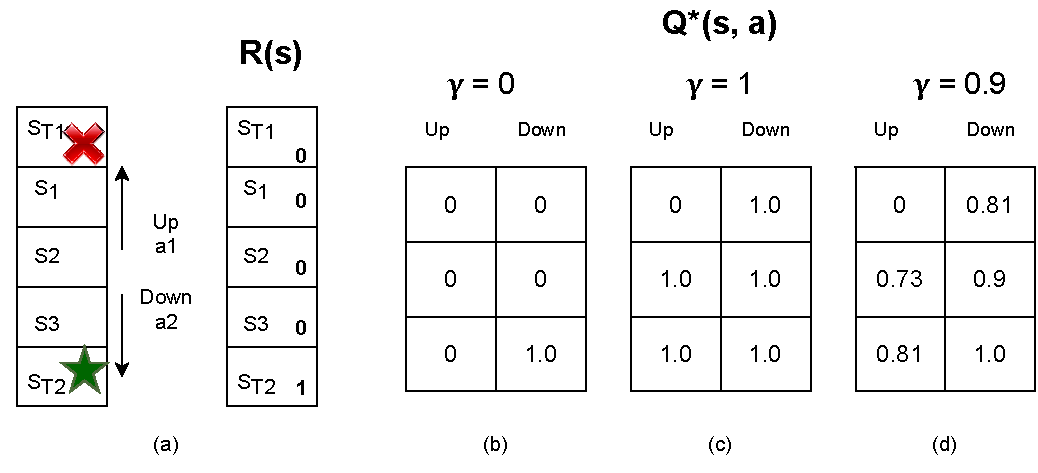
\includegraphics[height=2.5in]{figs/DRL-1d-Q_new}
\caption{
  Left: illustration of a simple MDP
  corresponding to a 1d grid world
  of 3 non-absorbing states and 2 actions.
  Right: optimal $Q$-functions for different values of $\gamma$.
\figbased{Figures 3.1, 3.2, 3.4 of \citep{Graesser2019}}.
}
\label{fig:Q1d}
\end{figure}

\section{Computing the value function and policy given a known world model}
\label{sec:planning}
\label{sec:rl-planning}
\label{sec:DPRL}

In this section, we discuss how
to compute the optimal value function (the \keywordDef{prediction problem})
and the optimal policy (the \keywordDef{control problem})
when the MDP model is known.
(Sometimes the term \keywordDef{planning} is used to refer
to computing the optimal policy, given a known model,
but planning can also refer to computing a sequence of actions,
rather than a policy.)
The algorithms we discuss are based on
\keywordDef{dynamic programming} (DP)
and \keywordDef{linear programming} (LP).

For simplicity, in this section, we assume
discrete state and action sets with $\gamma<1$.
However,
exact calculation of optimal policies often depends
polynomially on the sizes of $\calS$ and $\calA$,
and is intractable, for example, when the state space
is a Cartesian product of several finite sets.
This challenge is known as the
\keywordDef{curse of dimensionality}.
Therefore, approximations are typically needed,
such as using parametric or nonparametric representations of the value function or policy,
both for computational tractability and
for extending the methods to handle MDPs
with general state and action sets.
This requires the use of
\keywordDef{approximate dynamic programming} (ADP)
and \keywordDef{approximate linear programming} (ALP)
algorithms (see e.g., \cite{BertsekasRL}).

\eat{
using \keywordDef{dynamic programming} (\keywordDef{DP}).
The inputs to the algorithm
are the world model $p(s'|s,a)$
and reward function $R(s,a)$,
and the output is the optimal policy and 
its value function.
(This is called  \keywordDef{planning} using a known model.)
We assume the states and actions are discrete,
although similar methods can also be used in the linear-Gaussian case.
%(In fact the state space can be large, as long as $p(s'|s,a)$ is sparse.)
}

\subsection{Value iteration}
\label{sec:valueIter}
\label{sec:VI}

A popular and effective DP method for solving an MDP is
\keywordDef{value iteration} (VI).
Starting from an initial value function estimate $V_0$, the algorithm
iteratively updates the estimate by 
\begin{align}
\label{eqn:value-iteration}
V_{k+1}(s) = \max_a \left[
  R(s,a) + \gamma \sum_{s'} p(s'|s,a) V_k(s') \right]
\end{align}
Note that the update rule, sometimes called a
\keywordDef{Bellman backup},
is exactly the right-hand side of the Bellman optimality equation \cref{eqn:bellmanOptV}, with the unknown $\Vopt$ replaced by the current estimate $V_k$.
A fundamental property of \cref{eqn:value-iteration}
is that the update is a \keywordDef{contraction}:
it can be verified that
\begin{align}
\label{eqn:bellman-contraction}
\max_s |V_{k+1}(s) - \Vopt(s)| \le \gamma \max_s |V_k(s) - \Vopt(s)|
\end{align}
In other words, every iteration will reduce
the maximum value function error
by a constant factor.

$V_k$ will converge to $\Vopt$,
after which an optimal policy can be extracted using \cref{eqn:optPolFromV}.
In practice, we can often terminate VI
when $V_k$ is close enough to $\Vopt$,
since the resulting greedy policy wrt $V_k$
will be near optimal.
Value iteration can be adapted to learn the optimal action-value function $\Qopt$.

\subsection{Real-time dynamic programming (RTDP)}
\label{sec:RTDP}


In value iteration, we compute $\Vopt(s)$ and $\polopt(s)$
for all possible states $s$,
averaging over all possible next states $s'$ at each iteration,
as illustrated in \cref{fig:sutton-8-6}(right).
However, for some problems,
we may only be interested in the value (and policy)
for certain special starting states.
This is the case, for example, in
\keywordDef{shortest path problems} on graphs,
where we are trying to find the shortest
route from the current state to a goal state.
This can be modeled as an episodic MDP
by defining a transition matrix
$\ptran(s'|s,a)$ where
taking edge $a$ from node $s$ leads to the neighboring node $s'$
with probability 1.
The reward function is defined as $R(s,a)=-1$ for all states $s$
except the goal states,
which are modeled as absorbing
states.

In problems such as this, we can use a method
known as \keywordDef{real-time dynamic programming}
or \keywordDef{RTDP} \citep{Barto1995},
to efficiently compute an \keywordDef{optimal partial policy},
which only specifies what to do for the reachable states.
RTDP maintains a value function estimate $V$.
At each step, it performs a Bellman backup for the
current state $s$ by
$V(s) \assign \max_a \expectQ{R(s,a) + \gamma V(s')}{\ptran(s'|s,a)}$.
It picks an action $a$ (often with some exploration), reaches a next state $s'$,
and repeats the process.
%it picks an action $a$ for the current state $s$,
%according to $V$ (e.g., with an $\epsilon$-greedy exploration).
%It then performs a full
%expectation backup
%by computing $V(s) = \expectQ{R(s,a) + \gamma V(s')}{s'  \sim p(s'|s,a)}$.
%It then samples the next state $s'$,
%and repeats the process to update $V(s')$.
This can be seen as a form of the more general
\keywordDef{asynchronous value iteration},
that focuses its computational effort on parts of the state
space that are more likely to be reachable from the current state,
rather than synchronously updating all states at each iteration.
% Sutton p178

\subsection{Policy iteration}
\label{sec:policyIteration}

Another effective DP method for computing $\polopt$ is \keywordDef{policy iteration}.
It is an iterative algorithm that searches in the space
of deterministic policies until converging to an optimal policy.
Each iteration consists of two steps, \keywordDef{policy evaluation} and \keywordDef{policy improvement}.

The policy evaluation step, as mentioned earlier,
computes the value function for the current policy.
Let $\policy$ represent the current policy,
$\vv(s)=\Vpol(s)$ represent the value function encoded as a vector indexed by states,
$\vr(s) = \sum_a \policy(a|s) R(s,a)$ represent the reward vector,
and $\vT(s'|s) = \sum_a \policy(a|s) p(s'|s,a)$ 
represent the state transition matrix.
Bellman's equation for policy evaluation can be
written in the matrix-vector form as
\begin{align}
  \vv &= \vr + \gamma \vT \vv
  \label{eqn:policyEval}
  \end{align}
This is a linear system of equations in $|\cal{S}|$ unknowns.
We can solve it using matrix inversion:
$\vv = (\vI - \gamma \vT)^{-1} \vr$.
Alternatively, we can use value iteration
by computing
$\vv_{t+1} = \vr + \gamma \vT \vv_t$
until near convergence,
or some form of asynchronous variant
that is computationally more efficient.

Once we have evaluated $\Vpol$ for the current policy $\policy$,
we can use it to derive a better policy $\policy'$,
thus the name policy improvement.
To do this, we simply compute a deterministic
policy $\policy'$ that acts greedily with respect to $\Vpol$ in every
state, using
\be
\policy'(s) = \argmax_a \{R(s,a) + \gamma \expect{\Vpol(s')}\}
\ee
We can guarantee that $V_{\policy'} \ge \Vpol$.
This is called the \keywordDef{policy improvement theorem}.
To see this, define $\vr'$, $\vT'$ and $\vv'$ as before,
but for the new policy $\policy'$.
The definition of $\policy'$ implies
$\vr' + \gamma \vT' \vv \ge \vr + \gamma \vT \vv = \vv$,
where the equality is due to Bellman's equation.
Repeating the same equality, we have
\begin{align}
\vv &\le \vr' + \gamma \vT' \vv
\le \vr' + \gamma \vT' (\vr' + \gamma \vT' \vv)
\le \vr' + \gamma \vT' (\vr' + \gamma \vT' (\vr' + \gamma \vT' \vv) ) \le \cdots \\
&= (\vI + \gamma \vT' + \gamma^2 \vT'^2 + \cdots) \vr'
= (\vI - \gamma \vT')^{-1} \vr'
= \vv'
\end{align}

Starting from an initial policy $\policy_0$, policy iteration alternates
between policy evaluation ($E$)
and improvement ($I$) steps,
as illustrated below:
\begin{align}
\policy_0 \stackrel{E}{\ra} V_{\policy_0}
\stackrel{I}{\ra} \policy_1
\stackrel{E}{\ra} V_{\policy_1}
\cdots
\stackrel{I}{\ra} \polopt
\stackrel{E}{\ra} \Vopt
\end{align}
%where $E$ stands for policy evaluation and $I$ stands for policy improvement.
The algorithm stops at iteration $k$, if the policy $\policy_k$
is greedy with respect to its own value function $V_{\policy_k}$.
In this case, the policy is optimal.
Since there are at most $|\calA|^{|\calS|}$ deterministic policies,
and every iteration strictly improves the policy, the algorithm must converge after finite iterations.


%\label{sec:GPI}
In PI,
we alternate between policy evaluation (which involves multiple
iterations, until convergence of $\Vpol$),
and policy improvement.
In VI, we alternate between
one iteration of policy evaluation followed
by one iteration of policy improvement
(the ``$\max$'' operator in the update rule).
%In \keywordDef{generalized policy improvement} or \keywordDef{GPI},
We are in fact free to intermix any number of
these steps in any order.
The process will converge once the
policy is greedy wrt its own  value function.



\begin{figure}
\centering
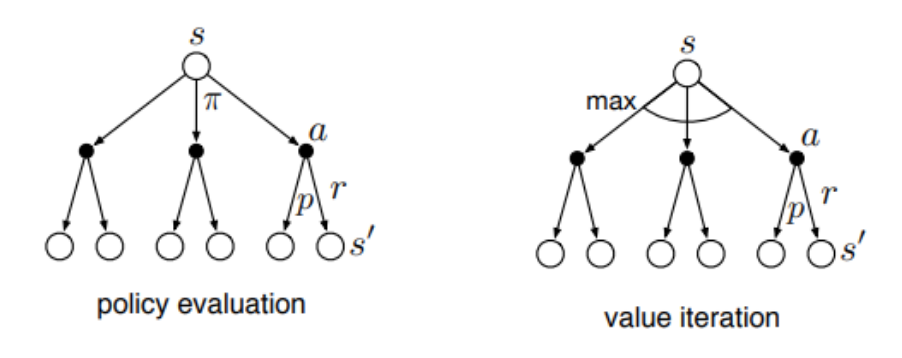
\includegraphics[height=1.5in]{figs/sutton-8-6-PI-VI}
\caption{
  Policy iteration vs value iteration represented as backup diagrams.
  Empty circles represent states, solid (filled) circles
  represent states and actions.
  \figbased{Figure 8.6 of \citep{Suttonv2}}.
}
\label{fig:sutton-8-6}
\end{figure}

Note that policy evaluation computes $\Vpol$
whereas value iteration computes $\Vopt$.
This difference is illustrated in \cref{fig:sutton-8-6},
using a \keywordDef{backup diagram}.
Here the root node represents any state $s$,
nodes at the next level represent state-action combinations
(solid circles),
and nodes at the leaves representing the set of possible
resulting next state $s'$ for each possible action.
In PE, we average over all actions according
to the policy, whereas in VI, we take the maximum over
all actions.

\section{Computing the value function  without knowing the world model}

In the rest of this chapter,
we assume the agent only has  access to samples from
the environment, $(s',r) \sim p(s',r|s,a)$.
We will show how to use these samples
to learn optimal value function and $Q$-function,
even without knowing the MDP dynamics.



\subsection{Monte Carlo estimation}
\label{sec:MCRL}

Recall that $\Vpol(s) = \expect{\return_t | s_t=s}$
is the sum of expected (discounted) returns from state $s$
if we follow policy $\pi$.
A simple way to estimate this is to rollout the policy,
and then compute the average
sum of discounted rewards.  The trajectory ends when we reach a terminal state, if
the task is episodic, or when the discount factor $\gamma^t$ becomes
negligibly small, whichever occurs first.
This is called \keywordDef{Monte Carlo estimation}.
We can use this to update our estimate of the value function as follows:
\begin{align}
\label{eqn:rl-td}
V(s_t) &\assign V(s_t) + \lr
\left[
 \return_t  - V(s_t)
  \right]
\end{align}
where $\lr$ is the learning rate, and the term in brackets is an error term.
We can use a similar technique to estimate
$\Qpol(s,a) = \expect{\return_t | s_t=s,a_t=a}$
by simply starting the rollout with action $a$.

We can use MC estimation of $Q$,  together with policy iteration
(\cref{sec:policyIteration}), to learn an optimal policy.
Specifically,
at iteration $k$,
we compute a new, improved policy using
$\policy_{k+1}(s) = \argmax_a Q_k(s,a)$,
where $Q_k$ is approximated using MC estimation.
This update can be applied to all the states visited
on the sampled trajectory.
This overall technique
is called \keywordDef{Monte Carlo control}.

To ensure this method converges to the optimal policy,
we need to collect data for every (state, action) pair,
at least in the tabular case,
since there is no generalization
across different values of $Q(s,a)$.
One way to achieve this is to use an $\epsilon$-greedy policy
 (see \cref{sec:epsGreedy}).
Since this is an on-policy algorithm,
the resulting method will converge
to the optimal $\epsilon$-soft policy,
as opposed to the optimal policy.
It is possible to use importance sampling
to estimate the value function for the optimal policy,
even if actions are chosen according to the $\epsilon$-greedy policy.
However, it is simpler to just gradually reduce $\epsilon$.
% Sutton p101

\subsection{Temporal difference (TD) learning}
\label{sec:TD}

The Monte Carlo (MC) method in \cref{sec:MCRL}
results in 
an estimator for $V(s)$ with very high variance,
since it has to unroll many trajectories, 
whose returns are a sum of many random rewards generated by stochastic state transitions.
%might yield very different returns.
In addition, it is limited to episodic tasks
(or finite horizon truncation of continuing tasks),
since it must unroll to the end of the episode
before each update step,
to ensure it reliably estimates the long term return.

In this section, we discuss a more efficient technique called
\keywordDef{temporal difference} or \keywordDef{TD} learning
\citep{Sutton88}.
The basic idea is to incrementally
reduce the Bellman error
%, which is the difference between the LHS and RHS of the Bellman equations,
for sampled states or state-actions,
based on transitions instead of a long trajectory.
More precisely, suppose we are to learn
the value function $\Vpol$ for a fixed policy $\policy$.
Given a state transition $(s_t,a_t,r_t,s_{t+1})$,
where $a_t \sim \policy(s_t)$,
we change the estimate $V(s_t)$ so that
it moves towards the  \keywordDef{target value}
$\targetV_t = r_t + \gamma V(s_{t+1}) \approx G_{t:t+1}$:
\begin{align}
V(s_t) &\assign V(s_t) + \lr
\left[
  \underbrace{r_t + \gamma V(s_{t+1}) - V(s_t)}_{\delta_t}
  \right]
%  &= (1-\lr) V(s_t) + \lr \big(r_t + \gamma V(s_{t+1}) \big) \notag
\end{align}
where $\lr$ is the learning rate.
(See \citep{Ryzhov2015} for ways to adaptively set the learning rate.)
The $\delta_t=y_t - V(s_t)$ term 
is known as the \keywordDef{TD error}.
A more general form of TD update
for parametric value function representations is
\begin{align}
\label{eqn:rl-td-approx}
\vw \assign \vw + \lr \left[
r_t + \gamma \Vapprox(s_{t+1})
  - \Vapprox(s_t) \right] \nabla_{\vw}\Vapprox(s_t)
\end{align}
we see that  \cref{eqn:rl-td} is a special case.
The TD update rule for evaluating $\Qpol$ is similar,
except we replace states with states and actions.

% Sutton and Bartoe p202

It can be shown that TD learning in the tabular case,
\cref{eqn:rl-td}, converges to the correct value function,
under proper conditions~\citep{BertsekasRL}.
%such as the the decay schedule of learning rate~\citep{BertsekasRL}.
However, it may diverge when using nonlinear function approximators,
as we discuss in \cref{sec:deadlytriad}.
The reason is that this update is a
``\keywordDef{semi-gradient}'',
which refers to the fact
that we only take the gradient wrt the  value function,
$\nabla_{\vw} V(\vs_t, \vw_t)$,
treating the target $U_t$ as constant.

The potential divergence of TD is also consistent with
the fact that \cref{eqn:rl-td-approx} does not correspond
to a gradient update
on any objective function, despite having
a very similar form to SGD (stochastic gradient descent).
Instead, it is an example of \keywordDef{bootstrapping},
%As mentioned in \cref{sec:rl-introl-valuebased},
%updates like \cref{eqn:rl-td} are based on
%the idea of \keywordDef{bootstrapping},
in which the estimate, $\Vapprox(s_t)$,
is updated to approach a target,
$r_t + \gamma \Vapprox(s_{t+1})$,
which is defined by the value function estimate itself.
This idea is shared by DP methods
like value iteration, although they rely on the
complete MDP model to compute an exact Bellman backup.
In contrast, TD learning can be viewed as using
sampled transitions to approximate such backups.
An example of a non-bootstrapping approach is the
Monte Carlo estimation in the previous section.
It samples a complete trajectory,
rather than individual transitions,
to perform an update;
this avoids the divergence issue,
but is  often much less
efficient.
\cref{fig:TD-MC-DP} illustrates the difference between
MC, TD, and DP.

\begin{figure}
\centering
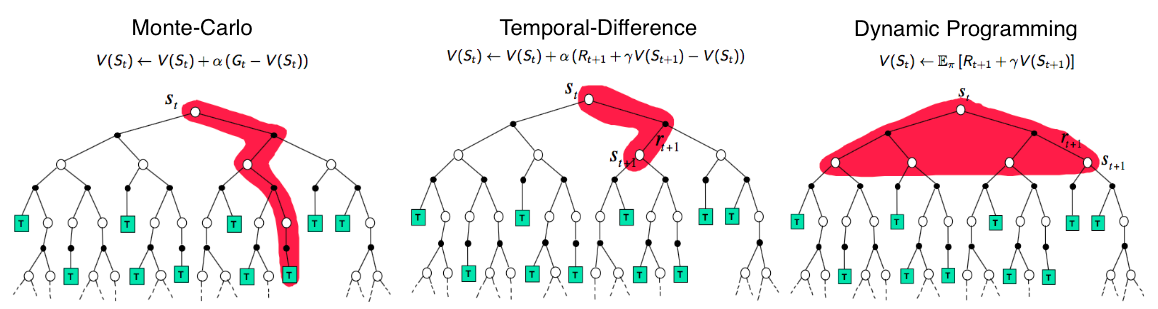
\includegraphics[height=1.5in]{figs/TD-MC-DP-backups}
\caption{
  Backup diagrams of $V(s_t)$ for Monte Carlo,
  temporal difference, and dynamic programming
  updates of the state-value function.
%  \figtaken{a figure from \citep{Silver2018L4}}.
%\figthanks{David Silver}.
\figthanks{Andy Barto}.
}
\label{fig:TD-MC-DP}
\end{figure}



\subsection{Combining TD and MC learning using TD($\lambda$)}
\label{sec:TDlambda}
\label{sec:nstep}

A key difference between TD and MC is
the way they estimate returns.
Given a trajectory
$\traj=(s_0,a_0,r_0,s_1,\ldots,s_T)$,
TD estimates the return from state $s_t$
by one-step lookahead,
$\return_{t:t+1} = r_t + \gamma V(s_{t+1})$,
where the return from time $t+1$ is replaced by
its value function estimate.
In contrast, MC waits until the end of the episode
or until $T$ is large enough,
then uses the estimate
$\return_{t:T} = r_t + \gamma r_{t+1} + \cdots + \gamma^{T-t-1} r_{T-1}$.
It is possible to interpolate between these by
performing an $n$-step rollout, and then using
the value function to approximate the return
for the rest of the trajectory,
similar to heuristic search (\cref{sec:heuristic}).
That is, we can use the \keywordDef{n-step return}
\begin{align}
\return_{t:t+n} = r_{t} + \gamma r_{t+1} + \cdots
+ \gamma^{n-1} r_{t+n-1} + \gamma^n V(s_{t+n})
\end{align}
For example, the 1-step and 2-step returns are given by
\begin{align}
  \return_{t:t+1} &= r_{t} + \gamma v_{t+1} \\
  \return_{t:t+1} &= r_{t} + \gamma r_{t+1} + \gamma^2 v_{t+2} \
  \end{align}
The corresponding $n$-step version of the TD update becomes
\begin{align}
  %V(s_t) \assign V(s_t) + \lr \left[\return_{t:t+n} - V(s_t)\right]
  \vw \assign \vw + \lr
  \left[\return_{t:t+n}  - \Vapprox(s_t) \right]
  \nabla_{\vw}\Vapprox(s_t)
\end{align}

Rather than picking a specific lookahead value, $n$,
we can take a weighted average of all possible values,
with a single parameter $\lambda\in[0,1]$,
by using
\begin{align}
\label{eqn:rl-gamma-return}
\return_{t}^{\lambda}
\defeq (1-\lambda) \sum_{n=1}^{\infty} \lambda^{n-1} \return_{t:t+n}
\end{align}
This is called the \keywordDef{lambda return}.
Note that these coefficients sum to one
(since $\sum_{t=0}^{\infty} (1-\lambda) \lambda^t = \frac{1-\lambda}{1-\lambda}=1$,
for $\lambda<1$),
so the return is a convex combination of $n$-step returns.
See \cref{fig:TDlambda} for an illustration.
We can now use $\return_t^{\lambda}$ inside the TD update
instead of $\return_{t:t+n}$;
this is called \keywordSpecial{TD$(\lambda)$}{TD(lambda)}.

Note that, if a terminal state is entered at step $T$ (as happens with episodic tasks),
then all subsequent $n$-step returns are equal to the conventional return, $G_t$.
Hence we can write
\begin{align}
  G_t^{\lambda} = (1-\lambda) \sum_{n=1}^{T-t-1}
  \lambda^{n-1} G_{t:t+n}
  \;
  + \lambda^{T-t-1} G_t
\end{align}
From this we can see that if $\lambda=1$, the $\lambda$-return
becomes equal to the regular MC return $G_t$.
If $\lambda=0$, the $\lambda$-return becomes equal to the
one-step return $G_{t:t+1}$ (since $0^{n-1}=1$ iff $n=1$),
so standard TD learning is often called
\keywordDef{TD(0) learning}.
This episodic form also gives us the following recursive equation
\be
G_t^{\lambda} = r_t + \gamma[(1-\lambda) v_{t+1} + \lambda G_{t+1}^{\lambda}]
\ee
which we initialize with $G_T=v_t$.
% https://github.com/google-deepmind/rlax/blob/master/rlax/_src/multistep.py#L34

\begin{figure}
\centering
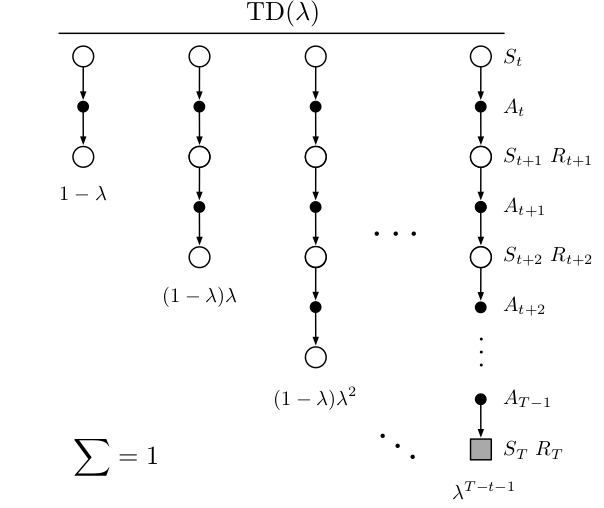
\includegraphics[height=2in]{figs/sutton-12-1}
\caption{
  The backup diagram for TD($\lambda$).
  Standard TD learning corresponds to $\lambda=0$,
  and standard MC learning corresponds to $\lambda=1$.
  \figtaken{Figure 12.1 of \citep{Suttonv2}}.
  \figthanks{Richard Sutton}.
}
\label{fig:TDlambda}
\end{figure}

\subsection{Eligibility traces}
\label{sec:eligibility}


An important benefit of using the geometric weighting
in \cref{eqn:rl-gamma-return}, as opposed to the $n$-step update,
is that
the corresponding TD learning update can be
efficiently implemented  through the use of
\keywordDef{eligibility traces},
even though $\return_{t}^{\lambda}$ is
a sum of infinitely many terms.
The eligibility term is a weighted sum of the gradients
of the value function:
\be
\vz_t = \gamma \lambda \vz_{t-1} + \nabla_{\vw} V_{\vw}(s_t)
\ee
(This trace term gets reset to 0 at the start of each episode.)
We replace the TD(0) update of
$\vw_{t+1} = \vw_t + \lr \delta_t \nabla_{\vw} V_{\vw}(s_t)$
with the TD($\lambda$) version to get
\be
\vw_{t+1} = \vw_t + \lr \delta_t \vz_t
\ee
See \citep{VanSeijen2016} for more details.

\section{SARSA: on-policy TD control}
\label{sec:SARSA}

TD learning is for policy evaluation,
as it estimates the value function for a fixed policy.
In order to find an optimal policy,
we may use the algorithm as a building block inside
generalized policy iteration (\cref{sec:policyIteration}).
In this case, it is more convenient
to work with the action-value function, $Q$, and
a policy $\policy$ that is greedy with respect to $Q$.
The agent follows $\policy$ in every step
to choose actions, and upon a transition $(s,a,r,s')$
the TD update rule is
\begin{align}
Q(s,a) \assign Q(s,a) + \lr \left[ r + \gamma Q(s',a') - Q(s,a) \right]
\label{eqn:rl-td-q}
\end{align}
where $a' \sim \policy(s')$ is the action
the agent will take in state $s'$.
After $Q$ is updated (for policy evaluation),
$\policy$ also changes accordingly as it is greedy
with respect to $Q$ (for policy improvement).
This algorithm, first proposed by \citep{Rummery1994},
was further studied and renamed to
\keywordDef{SARSA} by \citep{Sutton1996};
the name comes from its update rule that
involves an augmented transition $(s,a,r,s',a')$.

In order for SARSA to converge to $\Qopt$,
every state-action pair must be visited infinitely often,
at least in the tabular case,
since the algorithm only updates $Q(s,a)$
for $(s,a)$ that it visits.
One way to ensure this condition is to use a
``greedy in the limit with infinite exploration''
(\keywordDef{GLIE}) policy.
An example is the $\epsilon$-greedy policy,
with $\epsilon$ vanishing to $0$ gradually.
It can be shown that SARSA with a GLIE policy will
converge to $\Qopt$ and $\polopt$~\citep{Singh2000}.


\section{Q-learning: off-policy TD control}
\label{sec:Qlearning}

SARSA is an \keyword{on-policy} algorithm,
which means it learns the $Q$-function for the policy
it is currently using,
which is typically not the optimal policy,
because of the need to perform exploration.
However, with a simple modification,
we can convert this to an \keyword{off-policy}
algorithm that learns $\Qopt$,
even if a suboptimal or exploratory policy is used to choose actions.


\subsection{Tabular Q learning}

Suppose we modify SARSA by replacing the sampled next action
$a' \sim \policy(s')$ in \cref{eqn:rl-td-q}
with a greedy action:
$a' = \argmax_b Q(s',b)$.
This results in the following update
when a transition $(s,a,r,s')$ happens
\begin{align}
Q(s,a) \assign Q(s,a) + \lr \left[
  r + \gamma \max_{a'} Q(s',a') - Q(s,a) \right]
\label{eqn:Qlearning}
\end{align}
This is the update rule of \keywordDef{Q-learning}
for the tabular case~\citep{Watkins92}.


Since it is off-policy,
the method can use  $(s,a,r,s')$ triples
coming from any data source,
such as older versions of the policy,
or log data from an existing (non-RL) system.
If every state-action pair is visited infinitely often,
the algorithm provably converges to $\Qopt$
in the tabular case, with properly decayed learning rates~\citep{BertsekasRL}.
%See \cref{fig:oneStep} for a visual comparison of Q-learning,
%SARSA, TD and DP methods.
\cref{algo:Qlearning} gives a vanilla implementation of
Q-learning
%(with functiion approximation)
with $\epsilon$-greedy exploration.

\begin{algorithm}
\dontprintsemicolon
\caption{Tabular Q-learning with $\epsilon$-greedy exploration}
\label{algo:Qlearning}
Initialize value function $Q$ \\
\Repeat{converged}
       {
       Sample starting state $s$ of new episode \\
       \Repeat{state $s$ is  terminal}
       {
       Sample action
       $a=\begin{cases}
       \argmax_{b} Q(s,b), & \text{with probability $1-\epsilon$} \\
       \text{random action}, & \text{with probability $\epsilon$}
       \end{cases}$
               \\
       $(s',r) = \text{env.step}(a)$ \\
       Compute the TD error: $\delta = r + \gamma \max_{a'} Q(s',a') - Q(s,a)$ \\
       $Q(s,a) \leftarrow Q(s,a) + \lr \delta$ \\
       $s \leftarrow s'$ 
         }
}
\end{algorithm}

\eat{
\begin{algorithm}
\dontprintsemicolon
\caption{Q-learning with $\epsilon$-greedy exploration}
\label{algo:Qlearning}
Initialize value function parameters $\vw$ \\
\Repeat{converged}
       {
       Sample starting state $s$ of new episode \\
       \Repeat{state $s$ is  terminal}
       {
       Sample action
       $a=\begin{cases}
       \argmax_{b} \Qapprox(s,b), & \text{with probability $1-\epsilon$} \\
       \text{random action}, & \text{with probability $\epsilon$}
       \end{cases}$
               \\
       Observe state $s'$, reward $r$ \\
       Compute the TD error: $\delta = r + \gamma \max_{a'} \Qapprox(s',a') - \Qapprox(s,a)$ \\
       $\vw \assign \vw + \lr \delta \nabla_{\vw} \Qapprox(s,a)$ \\
           $s \assign s'$
         }
}
\end{algorithm}
}


%\subsection{Done states}
%\label{sec:done}

For terminal states, $s \in \calS^+$, we know that
$Q(s,a)=0$ for all actions $a$.
Consequently, for the optimal value function,
we have
$V^*(s) = \max_{a'} Q^*(s,a)=0$
for all terminal states.
%
When  performing online learning, we don't usually know
which states are terminal.
Therefore we assume that, whenever we take a step in the environment,
we get the next state $s'$ and reward $r$,
but also a binary indicator $\done(s')$ that tells us
if $s'$ is terminal.
In this case,  we set the target value in Q-learning
to $V^*(s')=0$ yielding the modified update rule:
\begin{align}
Q(s,a) \assign Q(s,a) + \lr \left[
  r + (1-\done(s')) \gamma \max_{a'} Q(s',a') - Q(s,a) \right]
\label{eqn:Qlearningdone}
\end{align}
For brevity, we will usually ignore this factor in the subsequent equations,
but it needs to be implemented in the code.

%\subsection{Example}
%\label{sec:Qlearning1d}


\begin{figure}
\centering
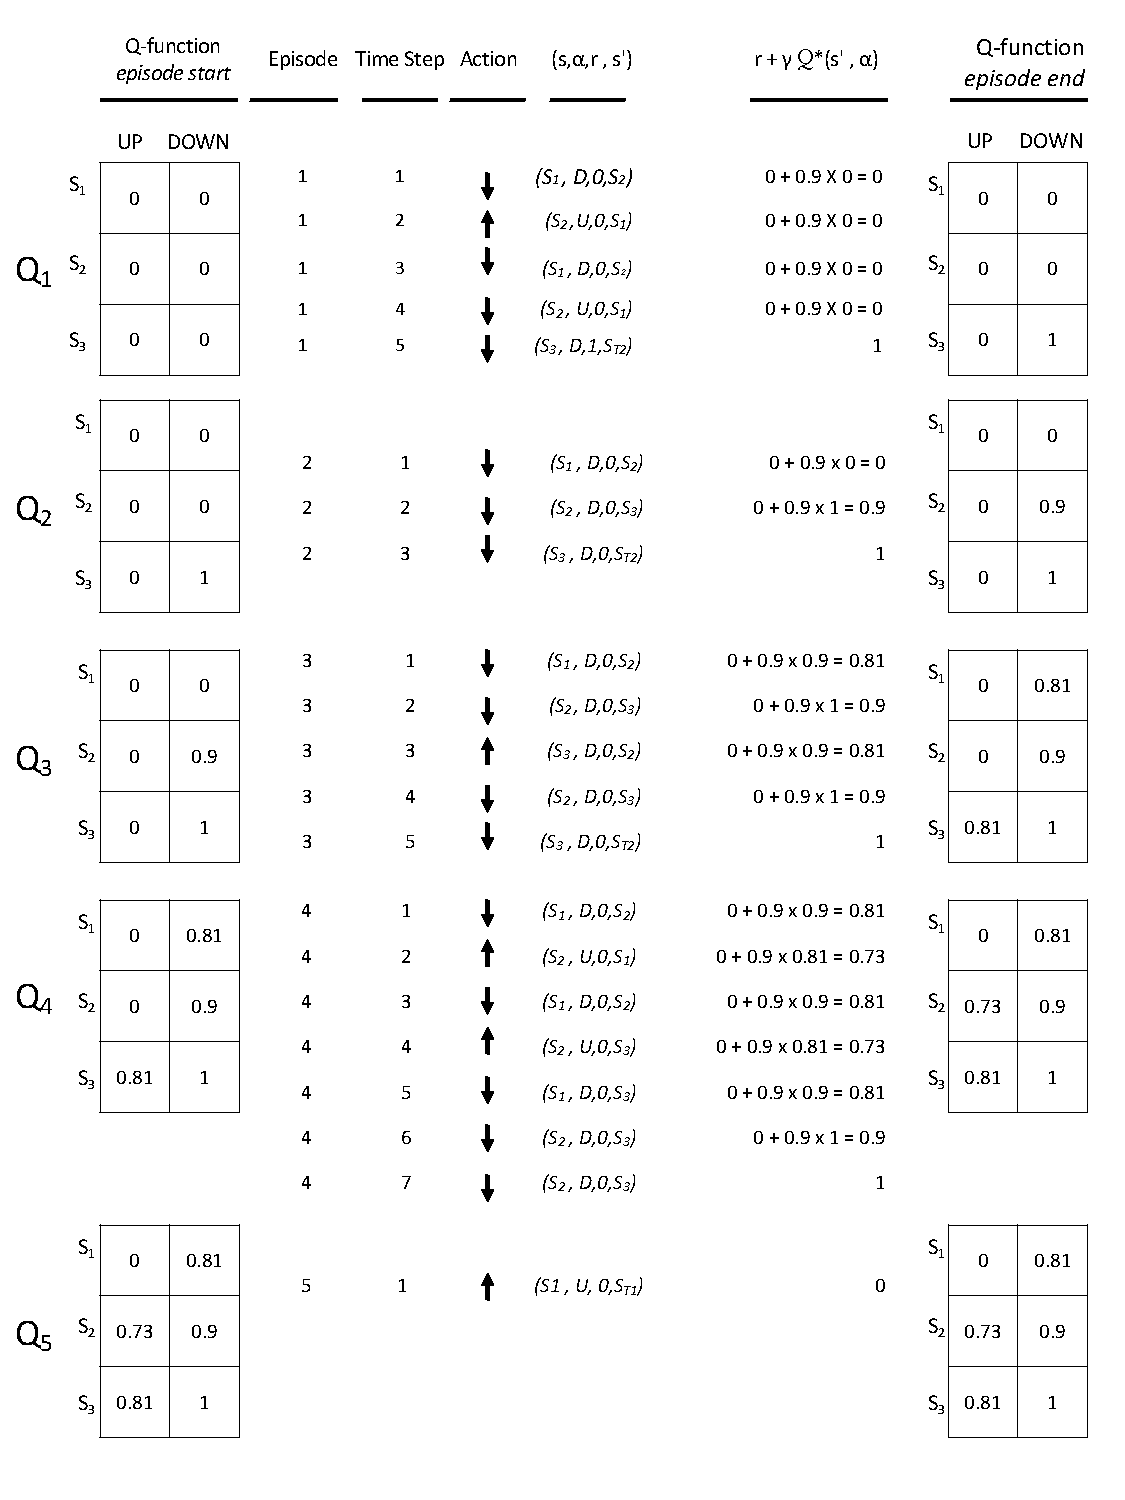
\includegraphics[height=5in]{figs/DRL-3-3}
\caption{
  Illustration of Q learning for one random trajectory
  in the 1d grid world
  in \cref{fig:Q1d} using $\epsilon$-greedy exploration.
  At the end of episode 1, we make a transition
  from $S_3$ to $S_{T2}$ and get a reward of $r=1$,
  so we estimate $Q(S_3,\downarrow)=1$.
  In episode 2, we make a transition from $S_2$ to $S_3$,
  so $S_2$ gets incremented by $\gamma Q(S_3,\downarrow)=0.9$.
  \figbased{Figure 3.3 of \citep{Graesser2019}}.
}
\label{fig:DRLTD}
\end{figure}

\cref{fig:DRLTD} gives an example
of Q-learning applied to the simple 1d grid world
from \cref{fig:Q1d}, using $\gamma=0.9$.
We show the $Q$-functon at the start and end of each episode,
after performing actions chosen by an $\epsilon$-greedy policy.
We initialize $Q(s,a)=0$ for all entries,
and use a step size of $\lr=1$.
At convergence, we have
$\Qopt(s,a) = r + \gamma \Qopt(s',a_*)$,
where $a_* = \downarrow$ for all states.




\subsection{Q learning with function approximation}
\label{sec:Qfn}

To make Q learning work with high-dimensional state spaces,
we have to replace the tabular (non-parametric) representation
with a parametric approximation, denoted $Q_{\vw}(s,a)$.
We can update this function using one or more steps of SGD
on the following loss function
\begin{align}
  \loss(\vw|\vs,a,r,\vs') &=
  \big( (r + \gamma \max_{a'} Q_{\vw}(\vs',a')) -   Q_{\vw}(\vs,a) \big)^2  
  \label{eqn:ynaive}
\end{align}
Since nonlinear functions need to be trained on minibatches
of data, we compute the average loss over multiple
randomly sampled
experience tuples (see \cref{sec:ER} for discussion)
  to get
  \begin{align}
\loss(\vw) &= \expectQ{\loss(\vw|\vs,a,r,\vs')}{(\vs,a,r,\vs') \sim U(\data)}
  \end{align}
%The random sampling helps reduce correlation between the samples.
%\begin{align}
%\vw  \assign \vw + \lr \left[
%  r + \gamma \max_{a'} Q_{_\vw}(s',a') - Q_{\vw}(s,a) \right]
%\nabla_{\vw} Q_{\vw}(s,a)
%\end{align}
See \cref{algo:Qfn} for the pseudocode.


\begin{algorithm}
\dontprintsemicolon
\caption{Q learning with function approximation and replay buffers}
\label{algo:Qfn}
Initialize environment state $\vs$,
network parameters $\vw_0$,
replay buffer $\data=\emptyset$,
discount factor $\gamma$,
step size $\eta$,
policy
$\pi_0(a|s) = \epsilon \text{Unif}(a)
+ (1-\epsilon) \delta(a=\argmax_a Q_{\vw_0}(s,a))$ \\
\For{iteration $k=0,1,2,\ldots$}
    {
      \For{environment step $s=0,1,\ldots,S-1$}
          {
            Sample action: $a \sim \pi_k(a|s)$ \\
            Interact with environment: $(s',r) = \text{env.step}(a)$ \\
            Update buffer: $\data \leftarrow \data \union \{ (s,a,s',r) \}$ 
          }
          $\vw_{k,0} \leftarrow \vw_k$ \\
          \For{gradient step $g=0,1,\ldots,G-1$}
              {
                Sample batch: $B \subset \data$ \\
                Compute error: $\loss(B,\vw_{k,g})
                = \frac{1}{|B|} \sum_{(s,a,r,s') \in B}
                \left[ Q_{\vw_{k,g}}(s,a) - (r + \gamma \max_{a'} Q_{\vw_k}(s',a')) \right]^2$\\
                Update parameters:
                $\vw_{k,g} \leftarrow \vw_{k,g} - \lr \nabla_{\vw_{k,g}}
                \loss(B,\vw_{k,g})$
              }
         $\vw_{k+1} \leftarrow \vw_{k,G}$ 
      }
\end{algorithm}

\subsubsection{Neural fitted Q}
\label{sec:NFQ}

The first approach of this kind
is known as \keywordDef{neural fitted Q iteration}
\citep{Riedmiller2005}, which corresponds to fully optimizing
$\loss(\vw)$ at each iteration (equivalent to using $G=\infty$
gradient steps).

\subsubsection{DQN}
\label{sec:DQN}

The influential
\keyword{deep Q-network} or \keyword{DQN}
paper of \citep{Mnih2015atari}
also used neural nets to represent the $Q$ function,
but performed a smaller number of gradient updates
per iteration.
Furthermore, they proposed to modify the target value
when fitting the $Q$ function in order to avoid
instabilities during training (see \cref{sec:deadly} for details).

The DQN method became famous since it was able  to train
agents that can outperform
humans when playing various Atari games from
the \keywordDef{ALE} (Atari Learning Environment)
benchmark \citep{Bellemare13}.
Here the input is a small color image,
and the action space corresponds to moving left, right, up or down,
plus an optional shoot action.\footnote{
%
For more discussion of ALE,
see \citep{Machado2018},
and for a recent extension to continuous actions
(representing joystick control),
see the CALE benchmark of \citep{Farebrother2024CALE}.
Note that DQN was not the first deep RL method to train
an agent from pixel input;
that honor goes to \citep{Lange2010},
who trained an autoencoder to embed images into low-dimensional latents,
and then used neural fitted Q learning (\cref{sec:NFQ})
to fit the $Q$ function.
}

Since 2015, many more extensions to DQN have been proposed,
with the goal of
improving performance in various ways,
either in terms of peak reward obtained,
or sample efficiency (e.g., reward obtained after only 100k steps
in the environment, as proposed in the \keywordDef{Atari-100k} benchmark
\citep{Atari100k}),
or training stability,
or all of the above.
We discuss some of these extensions in \cref{sec:DQNextensions}.



\eat{
\subsubsection{DQN}
\label{sec:DQN}


In this section, we discuss the seminal
\keywordDef{deep Q-network} or \keywordDef{DQN}
paper \citep{Mnih2015atari}.
The starting point is to consider the update
for the Q network parameters $\vw$
shown in \cref{algo:Qlearning}.
The gradient update corresponds to taking the gradient
of the following loss
\begin{align}
  \loss(\vw|\vs,a,r,\vs') &=
  \big( (r + \gamma \max_{a'} Q_{\vw}(\vs',a')) -   Q_{\vw}(\vs,a) \big)^2  
  \label{eqn:ynaive}
\end{align}
Since neural nets work best when trained on minibatches
of data, we compute the average loss by sampling
experience tuples (e.g., uniformly at random)
from
  the replay buffer $\data$
  (see \cref{sec:ER})
  to get
  \begin{align}
\loss(\vw) &= \expectQ{\loss(\vw|\vs,a,r,\vs')}{(\vs,a,r,\vs') \sim U(\data)}
  \end{align}
The random sampling helps reduce correlation between the samples.


\begin{algorithm}
\dontprintsemicolon
\caption{DQN (with target network)}
\label{algo:DQNtarget}
Initialize environment state $\vs$,
network parameters $\vw$,
target parameters $\overline{\vw} = \stopgrad(\vw)$,
replay buffer $\data=\emptyset$,
discount factor $\gamma$,
EMA rate $\rho$,
step size $\eta$
\\
\Repeat{converged}
       {
         Take action $a \sim \text{eps-greedy}(\vw)$\\
         $(\vs',r) = \text{step}(a, \vs)$ \\
         $\data := \data \union
         \{ (\vs, a, r, \vs') \}$ \\
         $\vs \assign \vs'$ \\
         Sample a minibatch $\calB = \{(\vs_j,a_j,r_j,\vs'_j)\}$
         from $\data$ \\
           $(\vw,\overline{\vw}) = \text{update}(\vw, \overline{\vw}, \calB)$
        }
.\\
$\text{def update}(\vw,\overline{\vw},\calB)$: \\
       Let $(\vs_j,a_j,r_j,\vs'_j)_{j=1}^B = \calB$ \\
$\targetV_{j} = \TargetV(r_j, \vs'_j; \overline{\vw})$ for $j=1:B$ \\
      $\loss(\vw) = \frac{1}{|\calB|} \sum_{(\vs_j, a_j, r_j, \vs'_j) \in
        \calB} (Q_{\vw}(\vs_j,a_j) - \stopgrad(\targetV_j))^2$\\
      $\vw \assign \vw - \lr_{\vw} \nabla \loss(\vw)$ // Gradient descent step \\
      $\overline{\vw} := \rho \overline{\vw} 
      + (1-\rho) \vw$       //EMA for  target network \\
    Return $\vw, \overline{\vw}$\\
\end{algorithm}
}


\subsubsection{Experience replay}
\label{sec:ER}
\label{sec:replay}

Since Q learning is an off-policy method, we can update the Q function
using any data source. This is particularly important when we use
nonlinear function approximation (see \cref{sec:Qfn}), which often needs a lot of data
for model fitting.
A natural source of data is data collected earlier in the trajectori
of the agent; this is called 
an \keywordDef{experience replay} buffer,
which stores  $(s,a,r,s')$ transition tuples into a buffer.
This can improve the stability and sample efficiency of learning,
and was
originally proposed in \citep{Lin1992}.

This modification has two advantages.
First, it improves data efficiency as every transition
can be used multiple times.
Second, it improves stability in training,
by reducing the correlation of the data samples
that the network is trained on,
since the training tuples do not have to come from
adjacent moments in time.
(Note that experience replay requires the use
of off-policy learning methods, such as Q learning,
since the training data is sampled from older
versions of the policy, not the current policy.)

%\subsubsection{Prioritized experience replay}
\label{sec:PER}

It is possible to replace the uniform sampling
from the buffer
with one that favors more
important transition tuples
that may be more informative about $Q$.
This idea is formalized in 
\citep{Schaul2016},
who develop a technique known as
\keywordDef{prioritized experience replay}.

\eat{
For example, we can sample transitions from $\data$
with probability
$p(s,a,r,s') \propto (|\delta| + \varepsilon)^{\eta}$,
%$p(i) = \frac{(|\delta_i| + \epsilon)^{\eta}}{(\sum_j |\delta_j|+\epsilon)^{\eta}}$,
where $\delta$ is the corresponding TD error
(under the current $Q$-function),
$\varepsilon > 0$ a hyperparameter
to ensure every experience is chosen
with nonzero probability,
and $\eta \geq 0$ controls the ``inverse temperature''
of the distribution (so $\eta=0$ corresponds to uniform sampling).
% Graesser p1110
}

\eat{
Consider the TD error for the $i$'th tuple $\tau_i$
\be
\delta_i = r_i + \gamma \max_{a'} Q_{\overline{\vw}}(s'_i, a')
 - Q_{\vw}(s_i,a_i)
\ee
Define the priority of $i$ as
\be
p_i = (\delta_i + \epsilon)^{\alpha}
\ee
where $\alpha \geq 0$ determines the degree of prioritization,
with $\alpha=0$ corresponding to no prioritization (uniform sampling).
Now define the probability of sampling $i$ as
\be
P(i) = \frac{p_i}{\sum_k p_k}
\ee
Sampling from this distribution will introduce bias relative
to the uniform distribution over the past $M$ samples in the replay buffer.
But we can correct this using importance sampling, as follows:
\begin{align}
  \expectQ{\loss(\tau)}{\text{Uniform}(\tau)}
  &= \sum_{i=1}^M \frac{1}{M} \loss(\tau_i) \\
  &= \sum_{i=1}^M P(\tau_i) \frac{1}{M P(\tau_i)} \loss(\tau_i) \\
  &= \expectQ{w(\tau) \loss(\tau)}{P(\tau)} 
  \end{align}
where we define the importance weight as
\be
w(\tau) = \left(\frac{1}{M P(\tau)} \right)^{\beta(t)}
\ee
Here $\beta(t)$ is a hyperparameter than starts off slightly larger than
0, to ensure that important experiences are not down-weighted too much,
and then is gradually increased to 1,
which results in an unbiased estimate.

%A distributed version of PER,
%known as \keywordDef{APE-X},
%is described in \citep{Horgan2018}.
}


\eat{
\subsubsection{Word of caution}

Unfortunately, when the function is nonlinear,
Q learning can become unstable; see \cref{sec:deadly} for details
of the problem and some solutions.
}






\subsubsection{The deadly triad}
\label{sec:offpolicyrl-deadlytriad}
\label{sec:deadlytriad}
\label{sec:deadlyTriad}
\label{sec:deadly}



\begin{figure}
\centering
\begin{subfigure}[b]{0.55\textwidth}
\centering
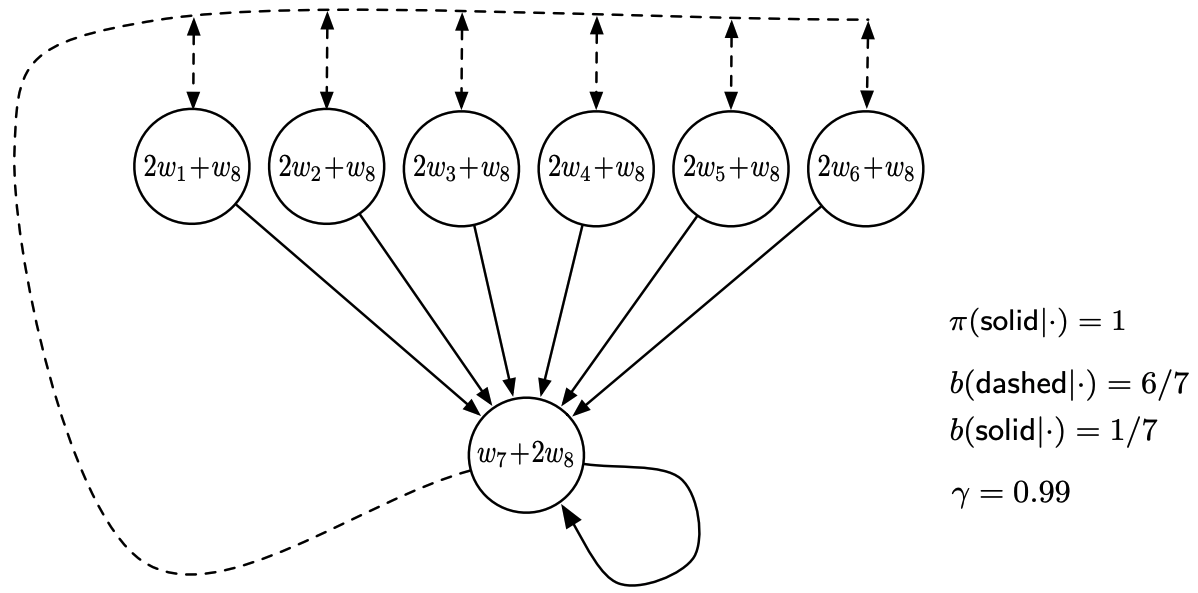
\includegraphics[height=1.75in]{figs/bairdExample}
\caption{ }
\label{fig:baird-example-mdp}
\end{subfigure}
~
\begin{subfigure}[b]{0.35\textwidth}
\centering
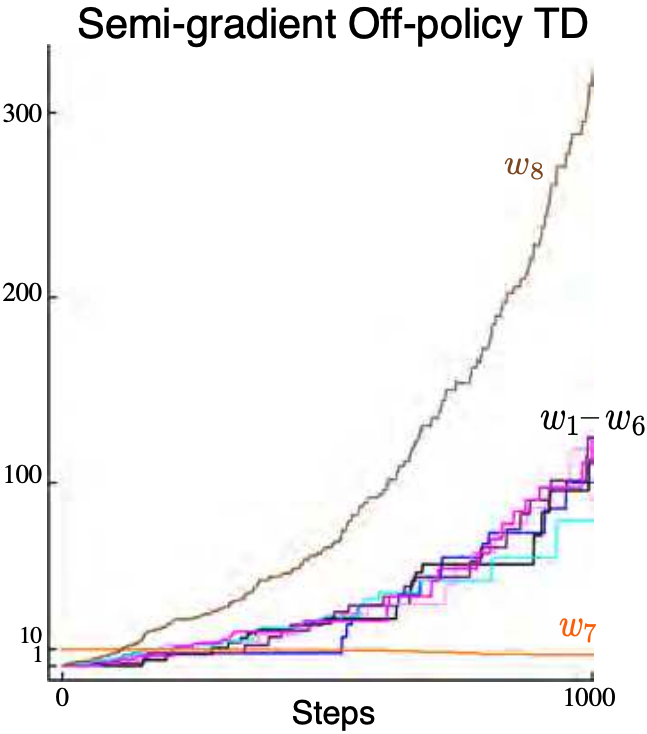
\includegraphics[height=1.75in]{figs/bairdExampleDivergence}
\caption{ }
\label{fig:baird-example-divergence}
\end{subfigure}
\caption{
(a) A simple MDP.
  (b) Parameters of the policy diverge over time.
\figtaken{Figures 11.1 and 11.2 of \citep{Suttonv2}}.
\figthanks{Richard Sutton}.
}
\label{fig:baird-example}
\end{figure}



The problem with the naive Q learning  objective in \cref{eqn:ynaive}
  is that it can lead to instability,
since the target we are regressing towards
uses the same parameters $\vw$ as the function we are updating.
So the network is ``chasing its own tail''.
Although this is fine for tabular models,  it can fail
for nonlinear models, as we discuss below.

In general, an RL algorithm can become unstable when it has
these three components:
function approximation (such as neural networks),
bootstrapped value function estimation (i.e., using TD-like methods instead of MC),
and off-policy learning (where the actions are sampled from some distribution
other than the policy that is being optimized).
This combination is known as \keywordDef{the deadly triad}
\citep{Sutton2015, Vanhasselt18}).
%It highlights another important challenge introduced by off-policy learning,
%and is a subject of ongoing research
%(e.g., \citep{Vanhasselt18,Kumar19}).

A classic example of this is the simple MDP depicted
in \cref{fig:baird-example-mdp}, due to \citep{Baird95}.
(This is known as \keywordDef{Baird's counter example}.)
It has 7 states and 2 actions.
Taking the dashed action takes the environment
to the 6 upper states uniformly at random,
while the solid action takes it to the bottom state.
The reward is 0 in all transitions,
and $\gamma=0.99$.
The value function $\Vapprox$ uses
a linear parameterization indicated by the expressions
shown inside the states, with $\vw\in\real^8$.
The target policies $\policy$ always chooses the
solid action in every state.
Clearly, the true value function, $\Vpol(s) = 0$,
can be exactly represented by setting $\vw=\vzero$.

Suppose we use a behavior policy $b$ to generate
a trajectory,
which chooses the dashed and solid actions
with probabilities $6/7$ and $1/7$, respectively,
in every state.
If we apply TD(0) on this trajectory,
the parameters diverge to $\infty$
(\cref{fig:baird-example-divergence}),
even though the problem appears simple.
In contrast, with on-policy data
(that is, when $b$ is the same as $\policy$),
TD(0) with linear approximation can be guaranteed to
converge to a good value function approximate~\citep{Tsitsiklis97}.
The difference is that with on-policy learning,
as we improve the value function, we also improve the policy,
so the two become self-consistent,
whereas with off-policy learning,
the behavior policy may not match the optimal
value function that is being learned,
leading to inconsistencies.


The divergence behavior is demonstrated in
many value-based bootstrapping methods, including TD, Q-learning,
and related approximate
dynamic programming algorithms,
where the value function is represented
either linearly (like the example above)
or nonlinearly~\citep{Gordon95,Tsitsiklis1997,Ostrovski2021}.
The root cause of these divergence phenomena
is that bootstrapping methods
typically are not minimizing a fixed objective function.  Rather, they
create a learning target using their own estimates, thus potentially
creating a self-reinforcing loop to push the estimates to infinity.
%In certain special cases, such a loop is not possible if data is
%on-policy, so one way to fix the problem is to apply off-policy
%correction methods discussed earlier.  
More formally, the problem is that
the contraction property in the tabular case
(\cref{eqn:bellman-contraction})
may no longer hold when $V$ is approximated by $\Vapprox$.

We discuss some solutions to the deadly triad problem below.


\subsubsection{Target networks}
\label{sec:targetNetwork}

One heuristic solution to the deadly triad,
proposed in the DQN paper,
is to use a  ``frozen'' 
\keywordDef{target network} computed at an earlier iteration
to define the target value for the DQN updates,
rather than trying to chase a constantly moving target.
Specifically, we maintain an extra copy
the $Q$-network, $Q_{\vw^-}$, 
with the same structure as $\Qapprox$.
This new $Q$-network is used
to compute bootstrapping targets
\be
\TargetV(r,\vs'; \vw^{-}) = r + \gamma \max_{a'} Q_{\vw^-}(\vs',a')
\ee
for training $\Qapprox$.
We can periodically set $\vw^{-} \assign \stopgrad(\vw)$,
usually after a few episodes,
where the stop gradient operator
is used to prevent autodiff propagating gradients back to $\vw$.
Alternatively, we can use
an exponential moving average (EMA)
of the weights,
i.e.,
we use 
 $\overline{\vw} = \rho \overline{\vw} + (1-\rho) \stopgrad(\vw)$,
where 
$\rho \ll 1$ ensures that $Q_{\overline{\vw}}$ slowly catches
up with $Q_{\vw}$.
(If $\rho=0$, we say that this is a \keywordDef{detached target},
since it is just a frozen copy of the current weights.)
The final loss  has the form
  \begin{align}
    \loss(\vw) &= \expectQ{\loss(\vw|\vs,a,r,\vs')}{(\vs,a,r,\vs') \sim U(\data)} \\
      \loss(\vw|\vs,a,r,\vs') &=
  (\TargetV(r,\vs';\overline{\vw}) -   Q_{\vw}(\vs,a))^2  
  \end{align}
%See \cref{algo:DQN} for the pseudocode.
Theoretical work justifying this technique is given
in  \citep{Fellows2023,Che2024}.


\eat{
\begin{algorithm}
\dontprintsemicolon
\caption{DQN (with target network)}
\label{algo:DQN}
Initialize environment state $\vs$,
network parameters $\vw$,
target parameters $\overline{\vw} = \stopgrad(\vw)$,
replay buffer $\data=\emptyset$,
discount factor $\gamma$,
EMA rate $\rho$,
step size $\eta$
\\
\Repeat{converged}
       {
         Take action $a \sim \text{eps-greedy}(\vw)$\\
         $(\vs',r) = \text{step}(a, \vs)$ \\
         $\data := \data \union
         \{ (\vs, a, r, \vs') \}$ \\
         $\vs \assign \vs'$ \\
         Sample a minibatch $\calB = \{(\vs_j,a_j,r_j,\vs'_j)\}$
         from $\data$ \\
           $(\vw,\overline{\vw}) = \text{update}(\vw, \overline{\vw}, \calB)$
        }
.\\
$\text{def update}(\vw,\overline{\vw},\calB)$: \\
       Let $(\vs_j,a_j,r_j,\vs'_j)_{j=1}^B = \calB$ \\
$\targetV_{j} = \TargetV(r_j, \vs'_j; \overline{\vw})$ for $j=1:B$ \\
      $\loss(\vw) = \frac{1}{|\calB|} \sum_{(\vs_j, a_j, r_j, \vs'_j) \in
        \calB} (Q_{\vw}(\vs_j,a_j) - \stopgrad(\targetV_j))^2$\\
      $\vw \assign \vw - \lr_{\vw} \nabla \loss(\vw)$ // Gradient descent step \\
      $\overline{\vw} := \rho \overline{\vw} 
      + (1-\rho) \vw$       //EMA for  target network \\
    Return $\vw, \overline{\vw}$\\
\end{algorithm}
}

\subsubsection{Two time-scale methods}

A general way to ensure convergence in off-policy
learning is to construct an objective function,
the minimization of which leads to a good value function approximation.
This is the basis of the
\keywordDef{gradient TD method} of \citep{Sutton2008,Maei2009,Ghiassian2020}.
%https://github.com/rlai-lab/Regularized-GradientTD
%see \citep[Ch.~11]{Suttonv2} for more information.
In practice, this can be achieved by  updating the target value in the TD update
more quickly than the value function itself;
this is known as a \keywordDef{two timescale optimization}
(see e.g., \citep{Yu2017TD,Zhang2019timescale,Hong2023}).
It is also possible to use a standard single timescale
method provided the target value is computed using a 
frozen \keyword{target network},
as discussed in \cref{sec:targetNetwork}.
See \citep{Fellows2023,Che2024} for details.

\subsubsection{Layer norm}

More recently, \citep{PQN} proved that just adding LayerNorm
\citep{Ba2016}
to the penultimate layer of the critic network,
just before the linear head,
is sufficient  to provably yield convergence of TD learning
even in the off-policy setting.
In particular, suppose the network has the form
$Q(s,a|\vw,\vtheta) = \vw^T \relu(\text{LayerNorm}(f(s,a;\vtheta)))$.
Since $||\text{LayerNorm}(f(s,a;\vtheta))|| \leq 1$, we have
$||Q(s,a|\vw,\vtheta) \leq ||\vw||$,
which means the magnitude of the output is always bounded,
as shown in \cref{fig:layerNorm}.
In \citep{PQN}, they prove this (plus $\ell_2$ regularization on $\vw$,
and a sufficiently wide penultimate layer)
is sufficient to ensure convergence 
of the value function estimate.



\begin{figure}
\centering
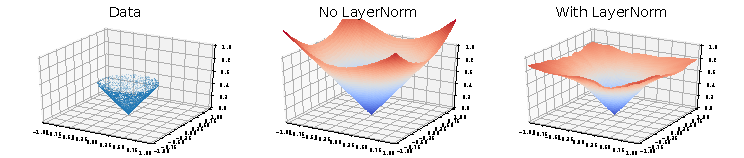
\includegraphics[height=1.5in]{figs/LayerNormFigure}
\caption{
  We generate a dataset (left) with inputs $\vx$
  distributed in a circle with radius 0.5 and labels $y = ||\vx||$.
  We then fit a two-layer MLP without LayerNorm (center)
  and with LayerNorm (right).
  LayerNorm bounds the values and prevents catastrophic overestimation
  when extrapolating.
  \figtaken{Figure  3 of \citep{Ball2023}}.
  \figthanks{Philip Ball}.
}
\label{fig:layerNorm}
\end{figure}



\eat{
% Bo Dai

  Thanks for asking! First, the deadly triad is offpolicy data + general function + TD. We can break the deadly triad by either use optimization based method to replace TD (e.g., LP-based RL with primal-dual solver https://arxiv.org/pdf/2001.01866), or use overparametrized general function (https://arxiv.org/abs/2405.21043). Second, linear value function with appropriate basis is also powerful. We had a series of work on developing the appropriate linear basis (representation) for RL (https://arxiv.org/pdf/2208.09515). Third, for convex Q function, I do not have general answer for general dynamics. However, for the multi-stage stochastic optimization  dynamic problem (https://arxiv.org/pdf/2112.00874), the Q is proved to be convex and TD converges.

 % Tom Zahavy.
  We had this paper on convex RL: https://openreview.net/pdf?id=ELndVeVA-TR, in this case we focus on value functions that are convex in the occupancy (while the value function is linear in it). These functions are quite popular for exploration/diversity/imitation so this convex setting is actually rich and meaningful. The problems are almost equivalent in terms of hardness results.

%  Hado van Hasselt.
  TD with linear value functions also suffers from the deadly triad in the off-policy case, though gradient TD (GTD) algorithms exist that do converge (in addition to alternatives Bo Dai mentioned above).

  Non-linear TD can additionally diverge even in the *on-policy* case. See, e.g., this classic paper by John Tsitsiklis and  @Benjamin Van Roy.
[Tsitsiklis1997]
  I conjecture that convexity in the parameters will not be sufficient to avoid this divergence.  If useful, I could try to construct a simple example to demonstrate this.  (I haven't checked carefully, maybe the example in the paper above is already convex.)

  However, for some problems even non-linear TD is guaranteed to converge.  For instance, this paper by Yann Ollivier
[Ollivier2018]
  that shows non-linear TD converges when the MDP is reversible, because then TD can be interpreted as stochastic gradient descent on a different objective (and therefore then inherits standard convergence properties of SGD).

Strict divergence does not always seem to happen, btw, when using a different optimiser, like ADAM, because this bounds the parameter updates.  This doesn't solve the issue, because the values can still get increasingly inaccurate when using an unstable update (we've called this phenomenon 'soft divergence' in the past).
}



\subsection{Maximization bias}

\begin{figure}
\centering
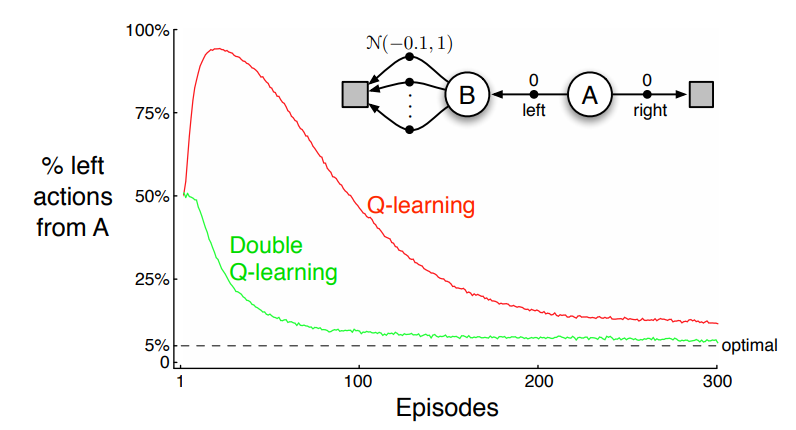
\includegraphics[height=1.5in]{figs/sutton-6-5}
\caption{
  Comparison of Q-learning and double Q-learning on a simple episodic
  MDP using $\epsilon$-greedy action selection with $\epsilon=0.1$.
  The initial state is A, and squares denote absorbing states.
The data are averaged over 10,000 runs.
\figtaken{Figure 6.5 of \citep{Suttonv2}}.
\figthanks{Richard Sutton}.
}
\label{fig:sutton-6-5}
\end{figure}

Standard Q-learning suffers from a problem
known as the \keywordDef{optimizer's curse} \citep{Smith2006},
or the \keywordDef{maximization bias}.
The problem refers to the simple statistical inequality:
$\expect{\max_a X_a} \geq \max_a \expect{X_a}$,
for a set of random variables $\{X_a\}$.
%where $r_i \sim p(R)$ are samples of $R$.
Thus, if we pick actions greedily according to their random scores $\{X_a\}$, we might pick a wrong action just because random noise makes it appealing.

% p135
\cref{fig:sutton-6-5} gives a simple example
of how this can happen in an MDP.
The start state is A.
The right action gives a reward 0 and terminates the episode.
The left action also gives a reward of 0,
but then enters state B,
from which there are many possible actions,
with rewards drawn from $\gauss(-0.1, 1.0)$.
Thus the expected return for any trajectory starting with the left
action is $-0.1$, making it suboptimal.
Nevertheless, the RL algorithm may pick   the left action
due to the maximization bias making B appear to have a positive value.

\subsubsection{Double Q-learning}
\label{sec:double}

One solution to avoid the maximization bias is to
use two separate $Q$-functions, $Q_1$ and $Q_2$,
one for selecting the greedy action,
and the other for estimating the corresponding $Q$-value.
%$\argmax_a Q_1(s,a)$,
%and the other of which is used to estimate the value
%of the chosen action, $Q_2(s,a_*)$.
%This estimate is unbiased,
%since $\expect{Q_2(s,a_*)}=Q(s,a_*)$.
%At each step, we perform the following update
In particular, upon seeing a transition $(s,a,r,s')$,
we perform the following update for $i=1:2$:
\begin{align}
  Q_i(s,a) &\assign Q_i(s,a) + \lr(\targetV_i(s,a) - Q_i(s,a)) \\
  \targetV_i(s,a) &= r + \gamma Q_{i}(s', \argmax_{a'} Q_{-i}(s', a'))
  \label{eqn:doubleQ}
%Q_1(s,a) \assign Q_1(s,a) + \lr \left[
%  r + \gamma Q_2\big(s', \argmax_{a'} Q_1(s',a')\big) -
%  Q_1(s,a) \right]
\end{align}
%% In particular, the training target for $Q_1$ becomes
%% $y_t =  r_{t+1} + \gamma Q_2(s_{t+1}, \argmax_a Q_1(s_{t+1},a))$.
%% (Alternatively, we can use
%% $y_t =  r_{t+1} + \gamma Q_1(s_{t+1}, \argmax_a Q_2(s_{t+1},a))$
%% as a training target for $Q_1$'
%% the choice is made randomly.)
So we see that $Q_1$ uses $Q_2$ to choose the best action
but uses $Q_1$ to evaluate it,
and vice versa.
%and may repeat the same update but with the roles
%of $Q_1$ and $Q_2$ swapped.
%We can also swap the roles of $Q_1$ and $Q_2$.
This technique is called
\keywordDef{double Q-learning} \citep{vanHasselt2010}.
\cref{fig:sutton-6-5} shows the benefits of
the algorithm over standard Q-learning
in a toy problem.

\subsubsection{Double DQN}
\label{sec:doubleDQN}


In \citep{vanHasselt2016}, they combine double Q learning
with deep Q networks (\cref{sec:DQN}) to get \keywordDef{double DQN}.
This modifies \cref{eqn:doubleQ}
to its gradient form, and then the current network for action
proposals, but the target network for action evaluation.
Thus  the  training target becomes
\be
\TargetV(r,\vs'; \vw, \overline{\vw}) = r + \gamma
Q_{\overline{\vw}}(\vs', \argmax_{a'} Q_{\vw}(\vs',a'))
\ee

In \cref{sec:TD3} we discuss an extension called
\keywordDef{clipped double DQN} which uses two Q networks
and their frozen copies
to define
the following target:
\be
\TargetV(r,\vs'; \vw_{1:2}, \overline{\vw}_{1:2}) = r + \gamma  \min_{i=1,2}
Q_{\overline{\vw}_i}(\vs',\argmax_{a'} Q_{\vw_i}(\vs',a'))
\ee
where $Q_{\overline{\vw}_i}$ is the target network for $Q_{\vw_i}$.
%We can derive a policy from the two networks by taking their average
%\be
%\pi(\vs,\vw) = \argmax_a \frac{1}{2} \sum_{i=1}^2 Q(\vs,a;\vw_i)
%\ee

\subsubsection{Randomized ensemble DQN}
\label{sec:REDQ}

The double DQN method is extended in
the \keywordDef{REDQ} (randomized ensembled double Q learning)
method of \citep{REDQ},
which uses
an ensemble of  $N>2$ Q-networks.
Furthermore, at each step, it draws a random
sample of $M \leq N$ networks, and takes the minimum over them
when computing the target value.
That is, it uses the following update
(see Algorithm 2 in appendix of \citep{REDQ}):
\be
\TargetV(r,\vs'; \vw_{1:N}, \overline{\vw}_{1:N})
= r + \gamma \max_{a'} \min_{i \in \calM} Q_{\overline{\vw}_i}(\vs',a')
\label{eqn:REDQtabular}
\ee
where $\calM$ is a random subset from the $N$ value functions.
The ensemble reduces the variance, and the minimum reduces
the overestimation bias.\footnote{
%
In addition, 
REDQ performs $G \gg 1$  updates of the value functions
for each environment step;
this  high \keywordDef{Update-To-Data} (UTD) ratio
(also called \keywordDef{Replay Ratio})
is critical for sample efficiency,
and is commonly used in model-based RL.
}
If we set $N=M=2$, we get a method
similar to clipped double Q learning.
(Note that REDQ is very similiar to the
\keywordDef{Random Ensemble Mixture} method of
\citep{Agarwal2020}, which was designed for offline RL.)



\eat{

See \cref{algo:REDQ} for some pseudocode for REDQ
for the tabular case.

\begin{algorithm}
\dontprintsemicolon
\caption{Tabular REDQ with experience replay}
\label{algo:REDQ}
Initialize $\{Q_i(s,a)\}_{i=1}^N$, $\overline{Q}_i=Q_i$ \\
$\hat{Q}(s,a) = \frac{1}{N} \sum_{i=1}^N Q_i(s,a)$\\
Initialize state $s$ \\
\Repeat{converged}
       {
         $a=\text{eps-greedy}(\hat{Q}(s,\cdot))$ \\
         $(s',r) = \text{step}(a,s)$\\
         $\data := \data \union \{ (s,a,r,s') \}$ \\
         \For{$G$ updates}
             {
               Sample a tuple $(s,a,r,s')$  from $\data$ \\
               Sample a set of $M$ indices $\calM \subseteq \{1,\ldots,N\}$ \\
               $Q_{\calM}(s,a) \defeq \min_{i \in \calM} \overline{Q}_i(s,a)$  \\
               Compute the  target 
               $\targetV(s,a) = r + \gamma \max_{a'} Q_{\calM}(s',a')$  \\
             \For{$i=1:N$}
                 {
                   $Q_i(s,a) \assign Q_i(s,a) + \lr(\targetV(s,a)-Q_i(s,a))$
                 }
             }
             $\hat{Q}(s,a) = \frac{1}{N} \sum_{i=1}^N Q_i(s,a)$\\
          $s \assign s'$
}
\end{algorithm}

}



\subsection{DQN extensions}
\label{sec:DQNextensions}

In this section, we discuss various extensions of DQN.

\subsubsection{Q learning for continuous actions}
\label{sec:QTopt}

Q learning is not directly applicable to continuous actions due to the need
to compute the argmax over actions.
An early solution to this problem,
based on neural fitted Q learning (see \cref{sec:NFQ}),
is proposed in \citep{Hafner2011}.
This became the basis of the 
DDPG algorithm of \cref{sec:DDPG},
which learns a policy to predict
the argmax.

An alternative  approach is to use gradient-free optimizers such as
the cross-entropy method to approximate the argmax.
The \keywordDef{QT-Opt} method of \citep{QTopt}
treats  the action vector $\va$ as a sequence of actions,
and optimizes one dimension at a time \citep{Metz2017}.
The  \keywordDef{CAQL} (continuous action $Q$-learning) method
of \citep{CAQL})
uses mixed integer programming to solve the $\argmax$ problem,
leveraging the \relu structure  of the $Q$-network.
The method of \citep{Seyde2022} quantizes each action dimension separately,
and then solves the argmax problem using methods inspired by  multi-agent RL.

  

\subsubsection{Dueling DQN}
\label{sec:duelingDQN}

The  \keywordDef{dueling DQN} method of \citep{Wang2016dueling},
learns a value function and an advantage function,
and derives the Q function, rather than learning it directly.
  This is helpful  when there are many actions with similar
$Q$-values, since the advantage $A(s,a)=Q(s,a)-V(s)$ focuses
  on the differences in value relative to a shared baseline.

In more detail, we define a network with $|A|+1$ output heads,
which computes  $A_{\vw}(\vs,a)$ for $a=1:A$ and
$V_{\vw}(\vs)$. We can then derive
\be
Q_{\vw}(\vs,a) = V_{\vw}(\vs) + A_{\vw}(\vs,a)
\ee
However, this naive approach ignores the following constraint
that holds for any policy $\pi$:
\begin{align}
\expectQ{A^{\pi}(s,a)}{\pi(a|s)}
&= \expectQ{Q^{\pi}(s,a) - V^{\pi}(s)}{\pi(a|s)} \\
&= V^{\pi}(s)  - V^{\pi}(s) = 0
\end{align}
Fortunately, for the optimal policy
$\pi^*(s) = \argmax_{a'} Q^*(s,a')$ we have
\begin{align}
0 
&= \expectQ{Q^*(s,a)}{\pi^*(a|s)}  - V^*(s) \\
&= Q^*(s, \argmax_{a'} Q^*(s,a')) - V^*(s) \\
&= \max_{a'} Q^*(s,a') - V^*(s) \\
&= \max_{a'} A^*(s,a')
\end{align}
Thus we can satisfy the constraint for the optimal policy
by subtracting off   $\max_a A(s,a)$ from the advantage head.
Equivalently we can compute the Q function using 
\be
Q_{\vw}(\vs,a) = V_{\vw}(\vs) + A_{\vw}(\vs,a) - \max_{a'} A_{\vw}(\vs,a')
\ee
In practice, the max is replaced by an average,
which seems to work better empirically.

\subsubsection{Noisy nets and exploration}
\label{sec:noisyDQN}
\label{sec:noisyNets}

Standard DQN relies on the epsilon-greedy strategy to perform exploration.
However, this will explore equally in all states,
whereas we would like to the amount of exploration
to be state dependent, to reflect the amount of uncertainty
in the outcomes of trying each action in that state
due to lack of knowledge (i.e., \keywordDef{epistemic uncertainty}
rather than aleatoric or irreducile uncertainty).
An early approach to this,
known as  \keywordDef{noisy nets} \citep{Fortunato2018},
added random noise to
the network weights to encourage exploration which is
temporally consistent within episodes.
More recent methods for exploration
are discussed in \cref{sec:exploreExploit}.
%are discussed in \cref{sec:intrinsicReward}.


\subsubsection{Multi-step DQN}
\label{sec:nsteps}

As we discussed in \cref{sec:TDlambda},
we can reduce the bias introduced by bootstrapping
by replacing TD(1) updates with TD($n$) updates,
where we unroll the value computation for $n$ MC steps,
and then plug in the value function at the end.
We can apply this to the DQN context by defining the target
\be
\targetV(s_0,a_0) = \sum_{t=1}^n \gamma^{t-1} r_t
 + \gamma^n \max_{a_n} Q_{\vw}(s_n, a_n)
 \ee
This can be implemented for episodic environments
by storing experience tuples of the form
\be
\tau = (s, a, \sum_{k=1}^n \gamma^{k-1} r_k, s_n, \done)
\ee
where $\done=1$ if the trajectory ended at any point
during the $n$-step rollout.
 
Theoretically this method is only valid if all the intermediate
actions, $a_{2:n-1}$, are sampled from the current optimal policy
derived from $Q_{\vw}$,
as opposed to some behavior policy,
such as epsilon greedy or some samples from the replay buffer
from an old policy.
In practice, we can just restrict sampling
to  recent samples from the replay buffer,
making the resulting method approximately on-policy.

Instead of using a fixed $n$, it is possible
to use a weighted combination of returns;
this is known as the  $Q(\lambda)$
  algorithm \citep{Peng1994,Kozuno2021}.

    

\eat{
\subsection{Putting it all together}

Many of the above methods can be combined for improved performance.
We give some examples of such hybrid methods below.
(Note that, besides combining various algorithmic pieces,
careful hyper-parameter tuning is critical for good results,
as discussed in \citep{Obando-Ceron2024}.)
}

\subsubsection{Rainbow}
\label{sec:rainbow}

The \keywordDef{Rainbow} method of \citep{rainbow}
combined 6 improvements to the vanilla DQN method,
as listed below.
(The paper is called ``Rainbow'' due to the color coding
of their results plot, a modified version of which is shown in
\cref{fig:rainbow}.)
At the time it was published (2018), this produced 
SOTA results on the Atari-200M benchmark.
The 6 improvements are as follows:
\begin{itemize}
\item Use \keyword{double DQN}, as in \cref{sec:doubleDQN}.

    \item  Use 
  \keyword{prioritized experience replay},  as in \cref{sec:PER}.

  
\item  Use the
categorical DQN (C51) (\cref{sec:C51}) 
distributional RL method.

  \item Use n-step returns (with $n=3$), as in \cref{sec:nsteps}.
  
\item Use \keyword{dueling DQN}, as in \cref{sec:duelingDQN}.

\item Use \keyword{noisy nets}, as in \cref{sec:noisyNets}.
\end{itemize}
Each improvement gives diminishing returns,
as can be see in \cref{fig:rainbow}.

\begin{figure}
\centering
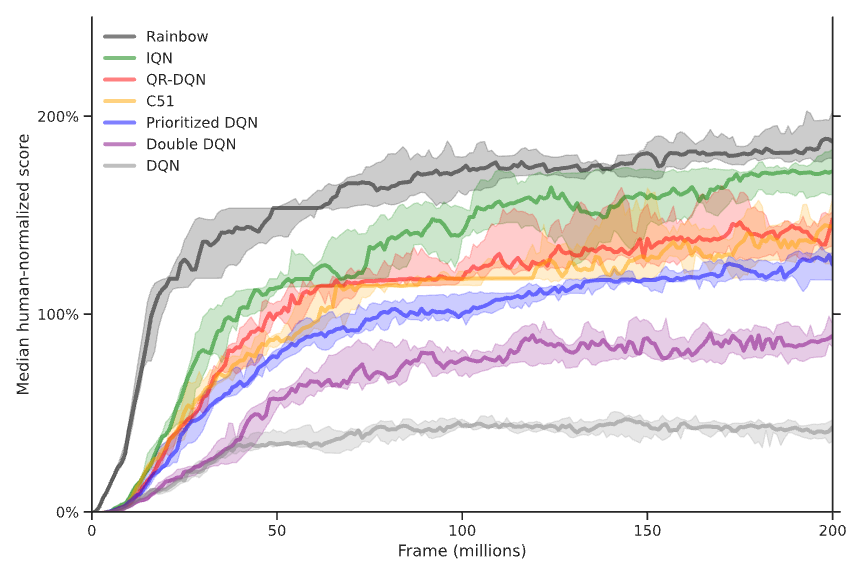
\includegraphics[height=1.5in]{figs/rainbow}
\caption{
  Plot of median human-normalized score over all 57 Atari games for
  various DQN agents.
  The yellow, red and green curves are distributional RL methods
  (\cref{sec:distributional}),
  namely categorical DQN (C51) (\cref{sec:C51})
  Quantile Regression DQN (\cref{sec:QRDQN}),
  and Implicit Quantile Networks \citep{IQN}.
  Figure from \url{https://github.com/google-deepmind/dqn_zoo}.
}
\label{fig:rainbow}
\end{figure}



Recently the ``Beyond the Rainbow'' paper \citep{beyond} proposed
several more extensions: 
\begin{itemize}
\item Use a larger CNN with residual connections,
  namely the Impala
  network from \citep{Espeholt2018}
  with the modifications (including the use of spectral normalization)
  proposed in
  \citep{Schmidt2021atari}.

  \item  Replace C51 with Implicit Quantile Networks \citep{IQN}.

  \item Use \keywordDef{Munchausen RL} \citep{Vieillard2020},
    which modifies
    the Q learning update rule by adding an entropy-like
    penalty.

  \item Collect 1 environment step from 64 parallel workers
    for each minibatch update (rather than taking many steps
    from a smaller number of workers).
\end{itemize}


\eat{
    \footnote{
    %
    The idea is as follows.
    First note that Q learning defines a greedy policy
    $\pi(a|s)=1$ iff $a = \argmax_{a'} Q(s,a')$,
    which we can convert to a stochastic policy
    $\pi(a|s) = \frac{\exp Q(s,a)}{\sum_{a'} Q(s,a')}$.
    Now consider the experience tuple
    $(s,a,r,s')$, so the Q learning
    target becomes $\targetV(s,a) = r + \max_{a'} Q^*(s',a')$.
Since $Q^*$ is unknown, we replace it with the current estimate
$Q_{\vw}(s',a')$ to get $\targetV(s,a) = r+q$ where $q=\max_{a'} Q_{\vw}(s',a')$.
However, this bootstrapping process can be unstable.
To help improve it, we can replace the target $r +q$ with
$r + \alpha \log \pi(a|s) + q$;
the motivation for this regularizer is that
the optimal policy should satisfy $\log \pi^*(a|s)$.
}
}


\subsubsection{Bigger, Better, Faster}
\label{sec:BBF}



At the time of writing this document (2024),
the SOTA on the 100k sample-efficient
Atari benchmark
\citep{Atari100k}
is obtained by the \keywordDef{BBF} algorithm of \citep{BBF}.
(BBF stands for ``Bigger, Better, Faster''.)
%This is arguably simpler than Rainbow.
It uses the following tricks,
in order of decreasing importance:
\begin{itemize}



\item Use a larger CNN with residual connections,
  namely a modified version of the Impala
  network from \citep{Espeholt2018}.

  \item Increase the \keywordDef{update-to-data} (UTD)
  ratio
  (number of times we update the Q function
  for every observation that is observed), in order to increase
  sample efficiency
  \citep{VanHasselt2019}.


\item Use a periodic soft reset of (some of) the network weights
to avoid loss of elasticity due to increased network updates, following the
\keywordDef{SR-SPR} method of \citep{DOro2022}.


\item Use n-step returns, as in \cref{sec:nsteps},
  and then gradually decrease (anneal) the n-step return from
 $n=10$ to $n=3$,
to reduce the bias over time.


\item Add weight decay.

\item Add a \keyword{self-predictive representation} loss
  (\cref{sec:self-predictive})
 to increase sample efficiency.

\item  Gradually increase the discount factor from
  $\gamma=0.97$ to $\gamma=0.997$,
  to encourage longer term planning once the model starts to be trained.\footnote{
  %
    The \keywordDef{Agent 57} method of  \citep{Badia2020}
  automatically learns the exploration rate and discount factor
  using a multi-armed bandit stratey,
  which lets it  be more exploratory or more exploitative,
  depending on the game. This resulted in super human performance
  on all 57 Atari games in ALE.
  However, it required 80 billion frames (environment steps)!
  This was subsequently reduced to the ``standard''
  200M frames in the \keywordDef{MEME} method of \citep{Kapturowski2022}.
  }


\item Drop noisy nets (which requires multiple network copies and thus slows
  down training due to increased memory use), since it does not help.

\item Use
  \keyword{dueling DQN} (see \cref{sec:duelingDQN}).

\item Use
  \keyword{distributional DQN}
  (see \cref{sec:distributional}).
  
%\item Use RNN models for the Q network,
%  as proposed in  the \keywordDef{R2D2} paper \citep{R2D2},
%  and used in many other papers.

\end{itemize}

\subsubsection{Other methods}

Many other methods have been proposed to reduce the sample complexity
of value-based RL while maintaining performance,
see e.g., the \keywordDef{MEME} paper of
\citep{Kapturowski2022}.





